\let\negmedspace\undefined
\let\negthickspace\undefined
\documentclass[journal]{IEEEtran}
\usepackage[a5paper, margin=10mm, onecolumn]{geometry}
\usepackage{tfrupee}
\usepackage{float}

\setlength{\headheight}{1cm}
\setlength{\headsep}{0mm}

\usepackage{gvv-book}
\usepackage{gvv}
\usepackage{cite}
\usepackage{amsmath,amssymb,amsfonts,amsthm}
\usepackage{algorithmic}
\usepackage{graphicx}
\usepackage{textcomp}
\usepackage{xcolor}
\usepackage{txfonts}
\usepackage{listings}
\usepackage{enumitem}
\usepackage{mathtools}
\usepackage{gensymb}
\usepackage{comment}
\usepackage[breaklinks=true]{hyperref}
\usepackage{tkz-euclide}
\usepackage[latin1]{inputenc}
\graphicspath{{figs/}}
\usepackage{color}
\usepackage{array}
\usepackage{longtable}
\usepackage{calc}
\usepackage{multirow}
\usepackage{hhline}
\usepackage{ifthen}
\usepackage{lscape}
\usepackage{circuitikz}



\begin{document}
\title{2.3.10}
\author{EE25BTECH11007- Aniket}
\maketitle
{\let\newpage\relax\maketitle}

\setlength{\intextsep}{10pt}
\textbf{Question}\\
If $\vec a$ and $\vec b$ are unit vectors, find the angle $\theta$ between $\vec a$ and $\vec b$
such that $\vec a-\sqrt{2}\,\vec b$ is a unit vector.\\

\textbf{Solution}\\
Since $\vec a$ and $\vec b$ are unit vectors,
\begin{gather}
\lVert \vec a \rVert = 1 \label{eq:unit-a}\\
\lVert \vec b \rVert = 1 \label{eq:unit-b}
\end{gather}
The condition that $\vec a-\sqrt{2}\,\vec b$ is also a unit vector gives
\begin{equation}
\big\lVert \vec a-\sqrt{2}\,\vec b \big\rVert = 1.
\label{eq:unit-cond}
\end{equation}
Squaring both sides:
\begin{equation}
\big\lVert \vec a-\sqrt{2}\,\vec b\big\rVert^{2}
= (\vec a-\sqrt{2}\,\vec b)^{\top}(\vec a-\sqrt{2}\,\vec b)=1.
\label{eq:norm-squared}
\end{equation}

\begin{equation}
(\vec a-\sqrt{2}\,\vec b)^{\top}(\vec a-\sqrt{2}\,\vec b)
= \vec a^{\top}(\vec a-\sqrt{2}\,\vec b)
\;-\;\sqrt{2}\,\vec b^{\top}(\vec a-\sqrt{2}\,\vec b).
\label{eq:distribute-outer}
\end{equation}

Using \eqref{eq:unit-a} and \eqref{eq:unit-b} and $\vec a^{\top}\vec b=\vec b^{\top}\vec a$:
\begin{equation}
1=(\vec a-\sqrt{2}\,\vec b)^{\top}(\vec a-\sqrt{2}\,\vec b)
= 1 -\sqrt{2}\,\vec a^{\top}\vec b \;-\;\sqrt{2}\,\vec a^{\top}\vec b \;+\;2
= 3 - 2\sqrt{2}\,(\vec a^{\top}\vec b).
\label{eq:combine}
\end{equation}

\begin{equation}
2\sqrt{2}\,(\vec a^{\top}\vec b)=2
\;\Longrightarrow\;
\vec a^{\top}\vec b=\frac{1}{\sqrt{2}}.
\label{eq:atb}
\end{equation}
Using the angle formula from dot product,
\begin{equation}
\cos\theta=\frac{\vec a^{\top}\vec b}{\lVert\vec a\rVert\,\lVert\vec b\rVert}
=\frac{1/\sqrt{2}}{1\cdot 1}=\frac{1}{\sqrt{2}},
\label{eq:costheta}
\end{equation}

\begin{equation}
\boxed{\;\theta=\frac{\pi}{4}=45^\circ\;}
\label{eq:final}
\end{equation}
\begin{figure}[H]
    \centering
    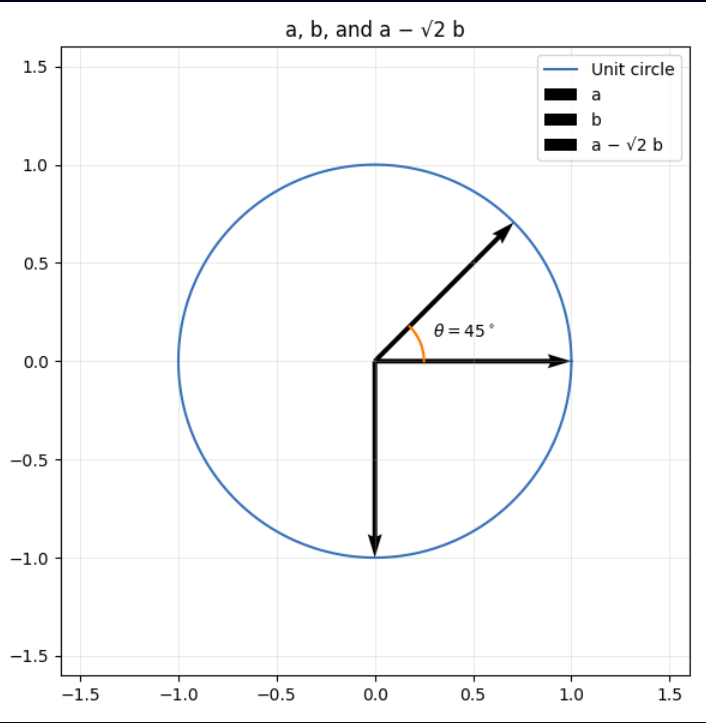
\includegraphics[width=\columnwidth]{figs/mg3plot.png}
\end{figure}
\end{document}